% !TeX program = pdflatex
%==============================================================================
%  Aula 09 --- Métricas para Classificação
%  VERSÃO DO ALUNO: texto para leitura autônoma, fora da sala.
%  (O roteiro de sala é "09 Metricas para Classificacao.tex".)
%==============================================================================
\documentclass[11pt,a4paper]{article}
\usepackage[aluno]{../../recursos/latex/estilo-notas}

\title{}
\date{}

\begin{document}
\cabecalhoaula{09}{Métricas para Classificação}{AME §7.4 e cap.~9; ISLP §4.4--4.5}

%==============================================================================
\section*{O que você vai aprender}
%==============================================================================
Ao final desta aula você deve ser capaz de:
\begin{itemize}[leftmargin=1.4cm]
  \item explicar por que a \emph{acurácia} pode ser uma péssima medida de
        desempenho;
  \item construir a \textbf{matriz de confusão} e definir sensibilidade,
        especificidade, precisão, VPN e $F_1$;
  \item derivar o \textbf{corte ótimo} sob uma perda assimétrica;
  \item ler uma \textbf{curva ROC}, interpretar a \textbf{AUC} e saber quando ela
        engana;
  \item escolher entre ajustar o corte, reponderar ou reamostrar em dados
        desbalanceados;
  \item distinguir \emph{classificar bem} de \emph{estimar bem probabilidades} e
        avaliar calibração.
\end{itemize}

\noindent
A Aula~08 terminou com um aviso: a acurácia pode enganar. Esta aula é o
desdobramento desse aviso. Comece por um caso concreto:

\begin{center}\itshape
  um teste de câncer que diz ``saudável'' para todo mundo acerta 99\% das vezes.\\
  Ele é bom?
\end{center}

\noindent
Obviamente não --- e o desconfortável é que a \emph{acurácia}, sozinha, não sabe
disso. Precisamos de medidas que enxerguem \emph{qual} erro foi cometido.

%==============================================================================
\section{Por que a acurácia não basta}
%==============================================================================
O risco 0--1 (Aula~08) trata \emph{todo} erro como igual. Mas:
\begin{itemize}[leftmargin=1.4cm,nosep]
  \item \textbf{Custos assimétricos:} num \emph{screening}, deixar de detectar um
        doente (falso negativo) é muito pior que um alarme falso (falso positivo).
  \item \textbf{Dados desbalanceados:} com 10 doentes em 1000, o classificador
        trivial $g\equiv 0$ tem acurácia 99\% --- e sensibilidade zero. Como
        métodos buscam aproximar o classificador de Bayes, eles \emph{tendem} a
        esse classificador inútil quando a classe é rara.
\end{itemize}

\begin{atencao}
A raiz do problema \textbf{não é} o desbalanceamento em si, mas o fato de que os
\emph{custos} dos erros são diferentes --- de modo que o classificador de Bayes
(que minimiza só a probabilidade de erro) deixa de ser o classificador desejado.
Tenha isso em mente: as ``correções'' abaixo são todas formas de codificar custos.
\end{atencao}

%==============================================================================
\section{Matriz de confusão e métricas}
%==============================================================================
Para classificação binária ($Y\in\{0,1\}$, ``1'' $=$ positivo), cruzamos predito
$\times$ verdadeiro. A matriz de confusão separa os dois tipos de acerto e os dois
tipos de erro, e é dela que sai toda métrica desta aula.

\begin{figure}[htbp]
  \centering
  \begin{tikzpicture}[font=\small, x=1cm, y=1cm]
    \node[font=\footnotesize\bfseries] at (2.6,1.35) {Verdadeiro};
    \node[font=\footnotesize] at (1.3,0.75)  {$Y=0$};
    \node[font=\footnotesize] at (3.9,0.75)  {$Y=1$};
    \node[font=\footnotesize\bfseries,rotate=90] at (-1.75,-1.3) {Predito};
    \node[font=\footnotesize] at (-0.75,-0.35) {$\ghat=0$};
    \node[font=\footnotesize] at (-0.75,-2.25) {$\ghat=1$};

    \fill[verdeesc!16] (0,-1.2) rectangle (2.6,0.5);
    \fill[vinho!20]    (2.6,-1.2) rectangle (5.2,0.5);
    \fill[vinho!20]    (0,-3.1) rectangle (2.6,-1.2);
    \fill[verdeesc!16] (2.6,-3.1) rectangle (5.2,-1.2);
    \draw (0,-3.1) rectangle (5.2,0.5);
    \draw (2.6,-3.1) -- (2.6,0.5);
    \draw (0,-1.2) -- (5.2,-1.2);

    \node[font=\bfseries] at (1.3,-0.2)  {VN};
    \node[font=\scriptsize] at (1.3,-0.75) {verdadeiro negativo};
    \node[font=\bfseries,vinho] at (3.9,-0.2)  {FN};
    \node[font=\scriptsize,vinho] at (3.9,-0.75) {falso negativo};
    \node[font=\bfseries,vinho] at (1.3,-2.1)  {FP};
    \node[font=\scriptsize,vinho] at (1.3,-2.65) {falso positivo};
    \node[font=\bfseries] at (3.9,-2.1)  {VP};
    \node[font=\scriptsize] at (3.9,-2.65) {verdadeiro positivo};

    % leituras por linha e por coluna
    \draw[-{Stealth[length=4pt]},vinho!80] (5.4,-2.1) -- (6.3,-2.1);
    \node[right,font=\scriptsize,align=left] at (6.35,-2.1)
      {\textbf{precisão} $=\dfrac{\text{VP}}{\text{VP}+\text{FP}}$\\[1pt]
       lê-se \emph{na linha}: dos que chamei\\de positivo, quantos acertei?};
    \draw[-{Stealth[length=4pt]},verdeesc!80] (3.9,-3.3) -- (3.9,-4.1);
    \node[below,font=\scriptsize,align=left] at (5.0,-4.15)
      {\textbf{sensibilidade} $=\dfrac{\text{VP}}{\text{VP}+\text{FN}}$\ \ lê-se
       \emph{na coluna}: dos positivos reais, quantos peguei?};
  \end{tikzpicture}
  \caption{A matriz de confusão e as duas leituras que mais confundem. Precisão e
  sensibilidade têm o \emph{mesmo} numerador (VP) e denominadores diferentes: uma
  divide pela \emph{linha} (o que você previu), a outra pela \emph{coluna} (o que
  de fato era). Saber qual é qual é metade da aula.}
  \label{fig:confusao}
\end{figure}

\noindent
As definições formais (cada uma estima uma probabilidade condicional populacional):
\begin{align*}
  \text{Sensibilidade (\emph{recall}):}\ & S=\frac{\text{VP}}{\text{VP}+\text{FN}}
    && \approx \Prob(\ghat=1\mid Y=1),\\
  \text{Especificidade:}\ & E=\frac{\text{VN}}{\text{VN}+\text{FP}}
    && \approx \Prob(\ghat=0\mid Y=0),\\
  \text{Precisão (VPP):}\ & P=\frac{\text{VP}}{\text{VP}+\text{FP}}
    && \approx \Prob(Y=1\mid \ghat=1),\\
  \text{Valor preditivo negativo:}\ & \text{VPN}=\frac{\text{VN}}{\text{VN}+\text{FN}}
    && \approx \Prob(Y=0\mid \ghat=0).
\end{align*}
A \textbf{estatística $F_1$} combina sensibilidade e precisão pela média harmônica:
\begin{equation}\label{eq:f1}
  F_1 = \frac{2}{1/S + 1/P} = \frac{2\,P\,S}{P+S}.
\end{equation}

\begin{ideia}
Por que média \emph{harmônica} e não aritmética? Porque a harmônica pune o
desequilíbrio. Um classificador com $S=1{,}0$ e $P=0{,}02$ --- que chama todo mundo
de positivo --- teria média aritmética $0{,}51$, respeitável; o $F_1$ dá $0{,}039$.
A média harmônica só é alta quando \emph{as duas} são altas, que é exatamente o que
se quer exigir.
\end{ideia}

\begin{atencao}
Todas essas quantidades devem ser calculadas no conjunto de \emph{validação/teste},
nunca no treino (senão superestimam o desempenho --- Aula~03). E note que
sensibilidade e especificidade \emph{não dependem da prevalência}, enquanto precisão
e VPN \emph{dependem}: o mesmo teste, aplicado a uma população com menos doentes,
tem a mesma sensibilidade e uma precisão pior. É por isso que um teste ``com 99\% de
sensibilidade'' pode, ainda assim, dar mais falsos que verdadeiros positivos numa
doença rara.
\end{atencao}

%==============================================================================
\section{Perdas assimétricas e o corte ótimo}
%==============================================================================
Para codificar custos diferentes, redefina o risco com pesos $l_0,l_1>0$:
\begin{equation}\label{eq:riscoassim}
  \risco(g) = l_1\,\Prob\big(Y\ne g(\X),\,Y=0\big)
            + l_0\,\Prob\big(Y\ne g(\X),\,Y=1\big),
\end{equation}
onde $l_0$ penaliza errar um positivo (FN) e $l_1$ penaliza errar um negativo (FP).

\begin{proposicao}[Corte ótimo sob perda assimétrica]\label{prop:corte}
O classificador que minimiza \eqref{eq:riscoassim} é
\[
  g(\x) = \1{\ \Prob(Y=1\mid\x) > \tfrac{l_1}{l_0+l_1}\ }.
\]
\end{proposicao}
\begin{proof}
Condicionando em $\x$, o custo esperado de prever $1$ é $l_1\Prob(Y=0\mid\x)$ e o de
prever $0$ é $l_0\Prob(Y=1\mid\x)$. Prevemos $1$ quando
$l_1\Prob(Y=0\mid\x) < l_0\Prob(Y=1\mid\x)$, isto é,
$l_1(1-\eta) < l_0\,\eta$ com $\eta=\Prob(Y=1\mid\x)$, o que dá
$\eta > l_1/(l_0+l_1)$. Como cada $\x$ é otimizado pontualmente, segue o resultado.
\end{proof}

\begin{ideia}
Eis a mensagem operacional: \textbf{mudar custos $=$ mudar o corte}. Com $l_0=l_1$
recuperamos o corte $1/2$ (Bayes). Se errar um positivo é dez vezes mais caro
($l_0=10 l_1$), o corte cai para $1/11\approx 0{,}09$ --- classificamos como
positivo com muito menos evidência. Repare no que \emph{não} é preciso fazer:
reajustar o modelo. As probabilidades estimadas continuam as mesmas; muda só o
número com que você as compara.
\end{ideia}

%==============================================================================
\section{Escolhendo o corte: curva ROC e AUC}
%==============================================================================
Um classificador \emph{plug-in} probabilístico gera uma \emph{família} de
classificadores variando o corte $K$: $g_K(\x)=\1{\widehat\Prob(Y=1\mid\x)\ge K}$.
Cada $K$ dá um par (sensibilidade, especificidade).

A \textbf{curva ROC} (\emph{Receiver Operating Characteristic}) traça a
sensibilidade contra $1-$especificidade à medida que $K$ varia de $1$ a $0$.
Propriedades:
\begin{itemize}[leftmargin=1.4cm,nosep]
  \item o canto superior esquerdo $(0,1)$ é o classificador perfeito;
  \item a diagonal é o ``palpite aleatório'';
  \item a \textbf{AUC} (área sob a curva) resume o desempenho em um número:
        $\text{AUC}=1$ é perfeito, $0{,}5$ é aleatório. Interpretação:
        probabilidade de o modelo dar \emph{score} maior a um positivo sorteado do
        que a um negativo sorteado.
\end{itemize}

\begin{figure}[htbp]
  \centering
  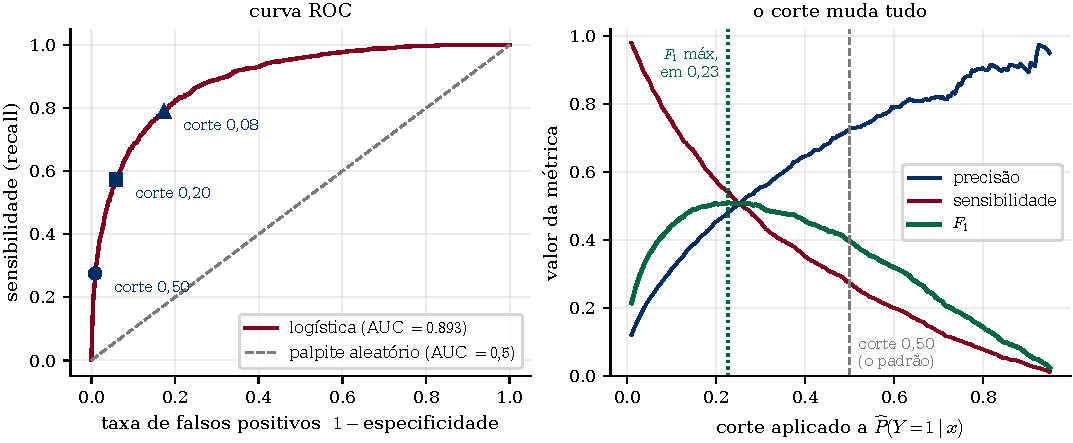
\includegraphics[width=\textwidth]{../../recursos/figuras/09-roc-metricas.pdf}
  \caption{Uma logística ajustada a um problema com prevalência de $7{,}9\%$,
  avaliada em $20\,000$ observações novas. \textbf{À esquerda}, a curva ROC: cada
  ponto é um corte diferente do \emph{mesmo} modelo. \textbf{À direita}, o que
  acontece com as métricas conforme o corte anda. No corte padrão $0{,}50$ a
  sensibilidade é baixíssima --- o modelo quase não chama ninguém de positivo. O
  $F_1$ é maximizado em $0{,}23$, não em $0{,}50$. E note o número que resume tudo:
  a acurácia no corte $0{,}50$ é $0{,}935$, contra $0{,}921$ do classificador que
  chuta ``negativo'' para todo mundo. Todo esse trabalho de modelagem comprou
  $1{,}4$ ponto percentual de acurácia --- e a acurácia, aqui, não é a pergunta
  certa.}
  \label{fig:roc}
\end{figure}

\begin{ideia}
A ROC/AUC avalia o \emph{ordenamento} dado pelo modelo \textbf{independentemente do
corte} --- útil para comparar classificadores antes de fixar custos. Já escolhido o
contexto, fixa-se $K$: critério comum é maximizar
$\text{Sensibilidade}+\text{Especificidade}$ (ponto mais próximo do canto
$(0,1)$), ou usar o corte da Prop.~\ref{prop:corte} se os custos são conhecidos.
\end{ideia}

\begin{atencao}
A curva ROC também deve ser construída na \emph{validação/teste}. E cuidado: em
dados muito desbalanceados a ROC engana, porque a taxa de falsos positivos tem no
denominador a classe majoritária --- que é enorme. Mil falsos positivos entre
$50\,000$ negativos mal movem o eixo horizontal, mas podem significar que apenas um
em cada dez alarmes é verdadeiro. A \emph{curva precisão--recall} não tem esse
problema e é mais informativa nesses casos.
\end{atencao}

%==============================================================================
\section{Lidando com dados desbalanceados}
%==============================================================================
Três famílias de estratégias (todas, no fundo, codificam custos):
\begin{description}[leftmargin=2.6cm,style=nextline]
  \item[Ajustar o corte] para métodos probabilísticos, basta mover $K$
        (Prop.~\ref{prop:corte}). Em geral é a solução mais limpa: não mexe no
        modelo, não descarta dados, não inventa observações.
  \item[Reponderar observações] dar peso maior à classe rara no treino, de modo que
        sua contribuição na função objetivo aumente (\texttt{class\_weight} no
        \texttt{scikit-learn}). Útil quando o método não estima $\Prob(Y=1\mid\x)$.
  \item[Re-amostrar] alterar artificialmente a prevalência: \emph{oversampling} da
        minoria (ex.: SMOTE) ou \emph{undersampling} da maioria.
\end{description}

\begin{atencao}
Repetindo a mensagem central: o ``problema'' não é o desbalanceamento, são os
\emph{custos desiguais}. Se os custos forem realmente iguais, um modelo bem
calibrado com corte $1/2$ pode ser o correto, mesmo desbalanceado. Não aplique
re-amostragem reflexivamente --- e note o efeito colateral: reamostrar
\textbf{destrói a calibração}, porque muda a prevalência que o modelo enxerga. Se
você precisa de probabilidades interpretáveis, prefira mexer no corte.
\end{atencao}

%==============================================================================
\section{Classificar bem $\neq$ estimar bem probabilidades}
%==============================================================================
Um classificador \emph{plug-in} pode estar muito perto do classificador de Bayes
\textbf{sem} que $\widehat\Prob\approx\Prob$: para a decisão, basta que
$\widehat\Prob(Y=1\mid\x)-K$ tenha o \emph{mesmo sinal} que
$\Prob(Y=1\mid\x)-K$. Ou seja, boa classificação não garante boa estimativa de
probabilidade.

Quando precisamos das \emph{probabilidades} em si (para ordenar riscos, decidir com
custos variáveis, ou inferência conformal), avaliamos com \textbf{regras de
pontuação próprias}, que são minimizadas pela probabilidade verdadeira:
\begin{itemize}[leftmargin=1.4cm,nosep]
  \item \textbf{Entropia cruzada / \emph{log-loss}}:
        $-\frac1n\sum_i\big[Y_i\log\widehat p_i + (1-Y_i)\log(1-\widehat p_i)\big]$
        (é a log-verossimilhança negativa da logística);
  \item \textbf{Score de Brier}:
        $\frac1n\sum_i (\widehat p_i - Y_i)^2$ (erro quadrático das
        probabilidades).
\end{itemize}

A ferramenta visual correspondente é a \textbf{curva de calibração}: agrupam-se as
observações por probabilidade predita e compara-se, em cada grupo, a média predita
com a frequência observada. Um modelo calibrado fica sobre a diagonal --- entre as
observações às quais ele deu $30\%$, cerca de $30\%$ devem ser positivas.

\begin{figure}[htbp]
  \centering
  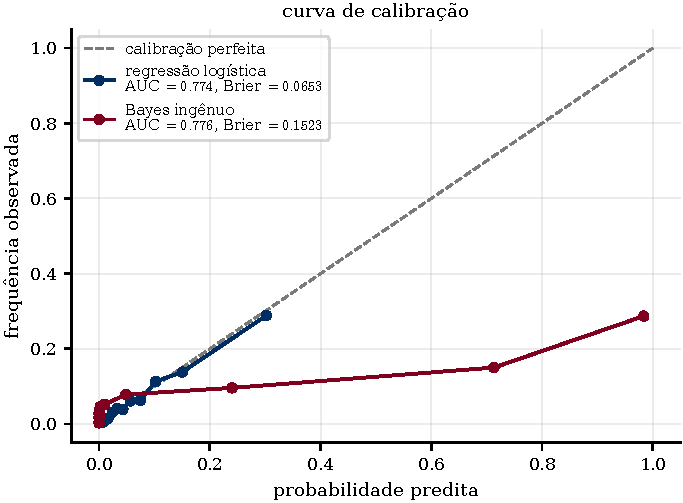
\includegraphics[width=0.62\textwidth]{../../recursos/figuras/09-calibracao.pdf}
  \caption{Duas curvas de calibração num problema com covariáveis fortemente
  correlacionadas --- cenário em que a hipótese do Bayes ingênuo é falsa. Os dois
  modelos \emph{ordenam} as observações praticamente igual (AUC $0{,}774$ contra
  $0{,}776$), mas o Bayes ingênuo chega a atribuir probabilidade $0{,}99$ a grupos
  em que só $29\%$ são positivos. O score de Brier registra a diferença que a AUC
  não vê: $0{,}065$ contra $0{,}152$, quase três vezes pior.}
  \label{fig:calibracao}
\end{figure}

\begin{ideia}
A Figura~\ref{fig:calibracao} é a demonstração literal do título desta seção. Se
você só precisa \emph{decidir} --- aprovar ou não um crédito, marcar ou não um
exame --- os dois modelos são equivalentes, e a AUC lhe diz isso corretamente. Se
você precisa \emph{do número} --- para calcular o valor esperado de uma decisão, ou
para comunicar risco a alguém --- o Bayes ingênuo é inutilizável, e só uma métrica de
calibração denuncia. Escolha a métrica pela pergunta que você vai responder.
\end{ideia}

\begin{observacao}
O motivo do descalibramento aqui é o da Aula~08: com covariáveis correlacionadas,
o produto $f(\x\mid Y=c)=\prod_j f(x_j\mid Y=c)$ do Bayes ingênuo conta a mesma
evidência muitas vezes, e o resultado é um modelo excessivamente confiante. Existem correções \emph{a posteriori} --- a
escala de Platt (ajustar uma logística sobre os \emph{scores}) e a regressão
isotônica --- disponíveis no \texttt{scikit-learn} como
\texttt{CalibratedClassifierCV}. Elas exigem dados próprios, separados do treino,
pelo motivo de sempre.
\end{observacao}

%==============================================================================
\section{Prática em Python}
%==============================================================================
\begin{lstlisting}
from sklearn.metrics import (confusion_matrix, classification_report,
                             roc_curve, roc_auc_score, brier_score_loss)

p = modelo.predict_proba(X_te)[:, 1]        # probabilidades estimadas

# 1. metricas no corte padrao 0,5
print(confusion_matrix(y_te, p >= 0.5))
print(classification_report(y_te, p >= 0.5))  # precisao, recall, F1 por classe

# 2. desempenho independente do corte
print("AUC:", roc_auc_score(y_te, p))
fpr, tpr, cortes = roc_curve(y_te, p)

# 3. qualidade das PROBABILIDADES, nao da decisao
print("Brier:", brier_score_loss(y_te, p))
\end{lstlisting}

\begin{atencao}
Ao escolher hiperparâmetros por validação cruzada (Aula~03), passe o
\texttt{scoring} certo para a sua pergunta: \texttt{"roc\_auc"} para ordenamento,
\texttt{"f1"} ou \texttt{"average\_precision"} para classes raras,
\texttt{"neg\_brier\_score"} ou \texttt{"neg\_log\_loss"} para probabilidades
calibradas. O padrão --- acurácia --- é justamente o que esta aula inteira
desaconselha.
\end{atencao}

O notebook \texttt{Aula prática 08} e o material \texttt{MatConf.pdf} exploram esses
conceitos com dados reais.

%==============================================================================
\section*{Resumo}
%==============================================================================
\begin{itemize}[leftmargin=1.4cm]
  \item Acurácia esconde \emph{qual} erro foi cometido; em classe rara, o
        classificador trivial já acerta quase tudo (Fig.~\ref{fig:roc}).
  \item A \textbf{matriz de confusão} (Fig.~\ref{fig:confusao}) gera sensibilidade e
        especificidade (leitura por coluna, independentes da prevalência) e precisão
        e VPN (leitura por linha, dependentes dela); $F_1$ \eqref{eq:f1} é a média
        harmônica de $P$ e $S$.
  \item Custos assimétricos $\Rightarrow$ o corte ótimo é $l_1/(l_0+l_1)$
        (Prop.~\ref{prop:corte}), não $1/2$. Mudar custos é mudar o corte, não o
        modelo.
  \item \textbf{ROC/AUC} avaliam o ordenamento, livres do corte; em desbalanceamento
        forte, prefira precisão--recall.
  \item Desbalanceamento: ajustar corte (limpo), reponderar, ou reamostrar (destrói
        calibração).
  \item \textbf{Classificar bem $\neq$ estimar bem probabilidades}
        (Fig.~\ref{fig:calibracao}): use \emph{log-loss}/Brier e curvas de
        calibração quando o número importar.
\end{itemize}

\paragraph{Leitura recomendada.} [AME] §7.4 (matriz de confusão e as métricas
derivadas), §9.1 (perdas assimétricas, cortes e dados desbalanceados --- de onde vem
a nossa Prop.~\ref{prop:corte}) e §9.2 (classificação \emph{versus} estimação de
probabilidades, o tema da nossa Figura~\ref{fig:calibracao}). [ISLP] §4.4.2 (matriz
de confusão no exemplo do \texttt{Default}, com uma discussão muito concreta de
sensibilidade em classe rara) e §4.4.3 (curva ROC e AUC).

\paragraph{Para praticar.} \texttt{recursos/listas/Lista de exercícios 08.pdf} traz
questões sobre as métricas desta aula.

\end{document}
